\section{Preventivo} %Meccanismi di controllo e rendicontazione
per ogni fase creare un prospetto delle ore secondo i ruoli ed economico. Per ognuno di essi anche uno riassuntivo.

Viene in seguito presentato il preventivo del costo del lavoro da svolgere con i dettagli sul costo di ogni singolo periodo.
Per identificare i diversi ruoli verranno utilizzate le sigle:
\begin{itemize}
	\item \textbf{Re}: responsabile di progetto;
	\item \textbf{Am}: amministratore di progetto;
	\item \textbf{An}: analista;
	\item \textbf{Pt}: progettista;
	\item \textbf{Pr}: programmatore;
	\item \textbf{Ve}: verificatore;
\end{itemize}
	\subsection{Periodo di analisi}
	Le ore indicate per questo periodo vengono riportate solo perché utili ai fini del documento, non saranno rendicontate nel budget finale richiesto in quanto il periodo di analisi è da considerare come investimento per il gruppo.
		\subsubsection{Prospetto orario}
		Nel periodo di analisi è prevista la seguente divisione oraria:
		\begin{longtable} {				
				>{}p{40mm}  
				>{}p{8mm}
				>{}p{8mm}
				>{}p{8mm}
				>{}p{8mm}
				>{}p{8mm}
				>{}p{8mm}
				>{}p{12mm}				
			}			
			\rowcolor{gray!50}
			\textbf{Nominativo} & \textbf{Re} & \textbf{Am} & \textbf{An} & \textbf{Pt} & \textbf{Pr} & \textbf{Ve} & \textbf{Totale}	\TBstrut \\ [2mm]
			Corrizzato Vittorio & 6 & 6 & 8 & - & - & 5 & 25 \TBstrut \\ [2mm]
			Dalla Libera Marco & 6 & - & 9 & 5 & - & 5 & 25 \TBstrut \\ [2mm]
			Rampazzo Marco & - & 8 & 12 & - & - & 5 & 25 \TBstrut \\ [2mm]
			Santagiuliana Vittorio & - & 5 & 12 & - & - & 8 & 25 \TBstrut \\ [2mm]
			Schiavon Rebecca & - & - & 13 & 5 & - & 7 & 25 \TBstrut \\ [2mm]
			Spreafico Alessandro & - & - & 12 & 5 & - & 8 & 25 \TBstrut \\ [2mm]
			Toffoletto Massimo & 8 & 7 & 5 & - & - & 5 & 25 \TBstrut \\ [2mm]
		\end{longtable}
		Rappresentata nel seguente grafico: \\
		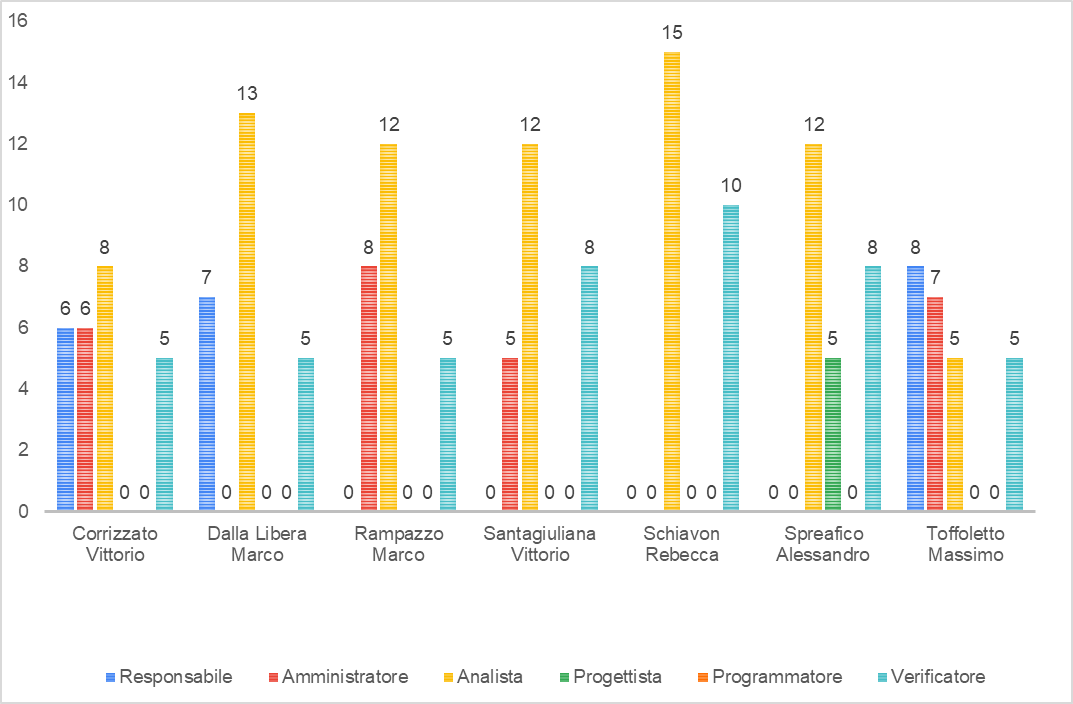
\includegraphics[width=\linewidth]{./img/Grafici/1.png}
	
		\subsubsection{Prospetto economico}
		Nel periodo di analisi sono previsti i seguenti costi:
		\begin{longtable} {
			>{}p{32mm}
			>{}p{20mm}
			>{}p{20mm}
		}
		\rowcolor{gray!50}
		
		\textbf{Ruolo} & \textbf{Ore} & \textbf{Costo} \TBstrut \\
		Responsabile & 20 & 600 \TBstrut \\
		Amministratore & 26 & 520 \TBstrut \\
		Analista & 71 & 1562 \TBstrut \\
		Progettista & 15 & 330 \TBstrut \\
		Programmatore & 0 & 0 \TBstrut \\
		Verificatore & 43 & 645 \TBstrut \\
		\textbf{Totale} & \textbf{175}& \textbf{3657} \TBstrut \\		
		\end{longtable}
		Rappresentati nel seguente grafico: \\
		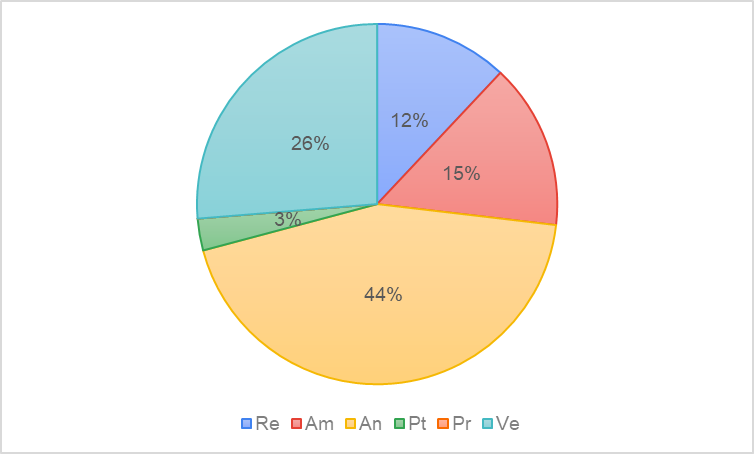
\includegraphics[width=\linewidth]{./img/Grafici/2.png}
\subsection{Periodo di progettazione architetturale}
	\subsubsection{Prospetto orario}
	Nel periodo di analisi è prevista la seguente divisione oraria:
	\begin{longtable} {				
		>{}p{40mm}  
		>{}p{8mm}
		>{}p{8mm}
		>{}p{8mm}
		>{}p{8mm}
		>{}p{8mm}
		>{}p{8mm}
		>{}p{12mm}				
	}			
	\rowcolor{gray!50}
	\textbf{Nominativo} & \textbf{Re} & \textbf{Am} & \textbf{An} & \textbf{Pt} & \textbf{Pr} & \textbf{Ve} & \textbf{Totale}	\TBstrut \\ [2mm]
	Corrizzato Vittorio & - & - & 6 & 10 & 5 & 7 & 28 \TBstrut \\ [2mm]
	Dalla Libera Marco & - & 5 & 7 & - & 7 & 9 & 28 \TBstrut \\ [2mm]
	Rampazzo Marco & 6 & - & - & 9 & 8 & 5 & 28 \TBstrut \\ [2mm]
	Santagiuliana Vittorio & - & - & - & 14 & 5 & 9 & 28 \TBstrut \\ [2mm]
	Schiavon Rebecca & 7 & - & - & - & 9 & 12 & 28 \TBstrut \\ [2mm]
	Spreafico Alessandro & - & 5 & 5 & - & 10 & 8 & 28 \TBstrut \\ [2mm]
	Toffoletto Massimo & - & - & 6 & 5 & 7 & 10 & 28 \TBstrut \\ [2mm]
	\end{longtable}
	Rappresentata nel seguente grafico: \\
	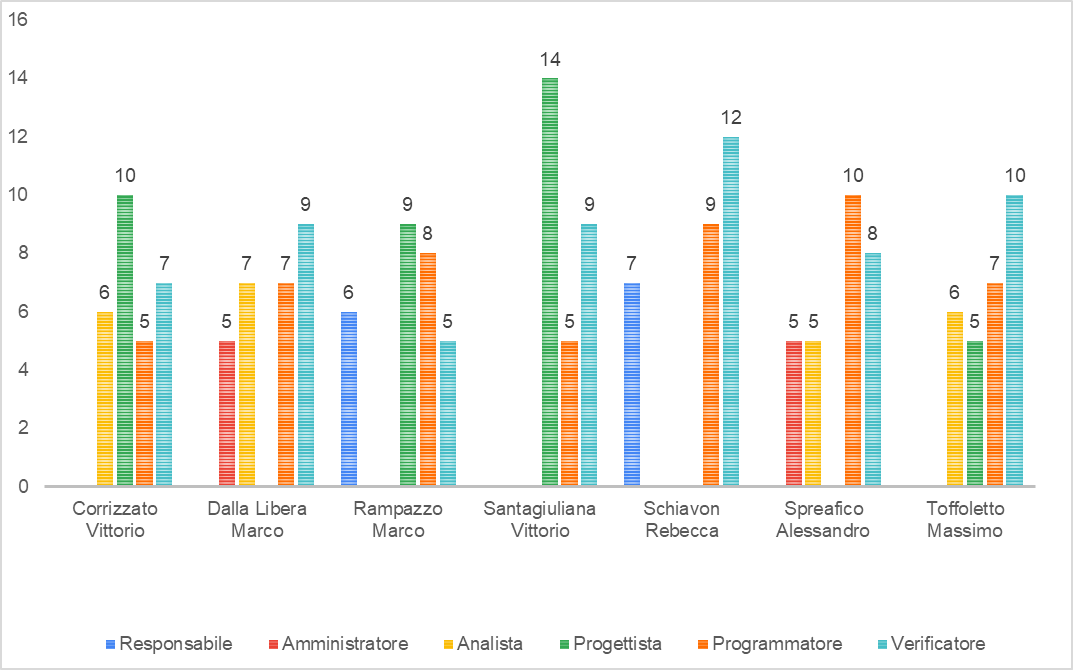
\includegraphics[width=\linewidth]{./img/Grafici/3.png}

\subsubsection{Prospetto economico}
Nel periodo di progettazione architetturale sono previsti i seguenti costi:
\begin{longtable} {
		>{}p{32mm}
		>{}p{20mm}
		>{}p{20mm}
	}
	\rowcolor{gray!50}
	
	\textbf{Ruolo} & \textbf{Ore} & \textbf{Costo} \TBstrut \\
	Responsabile & 13 & 390 \TBstrut \\
	Amministratore & 10 & 200 \TBstrut \\
	Analista & 24 & 528 \TBstrut \\
	Progettista & 38 & 836 \TBstrut \\
	Programmatore & 51 & 765 \TBstrut \\
	Verificatore & 60 & 900 \TBstrut \\
	\textbf{Totale} & \textbf{196}& \textbf{3619} \TBstrut \\		
\end{longtable}	
Rappresentati nel seguente grafico: \\
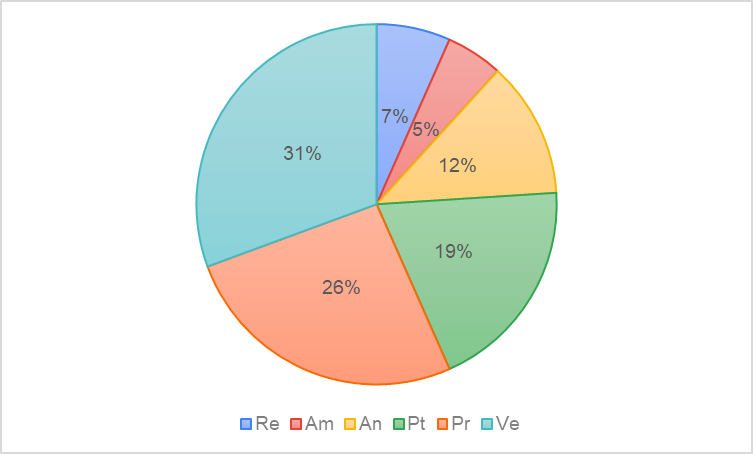
\includegraphics[width=\linewidth]{./img/Grafici/4.png}

\subsection{Periodo di progettazione dettaglio e codifica}
\subsubsection{Prospetto orario}
Nel periodo di progettazione dettaglio e codifica è prevista la seguente divisione oraria:
\begin{longtable} {				
		>{}p{40mm}  
		>{}p{8mm}
		>{}p{8mm}
		>{}p{8mm}
		>{}p{8mm}
		>{}p{8mm}
		>{}p{8mm}
		>{}p{12mm}				
	}			
	\rowcolor{gray!50}
	\textbf{Nominativo} & \textbf{Re} & \textbf{Am} & \textbf{An} & \textbf{Pt} & \textbf{Pr} & \textbf{Ve} & \textbf{Totale}	\TBstrut \\ [2mm]
	Corrizzato Vittorio & - & - & 9 & 23 & 22 & - & 54 \TBstrut \\ [2mm]
	Dalla Libera Marco & 9 & - & 6 & 15 & 15 & 9 & 54 \TBstrut \\ [2mm]
	Rampazzo Marco & - & 5 & - & 23 & 18 & 8 & 54 \TBstrut \\ [2mm]
	Santagiuliana Vittorio & 8 & - & - & 20 & 15 & 11 & 54 \TBstrut \\ [2mm]
	Schiavon Rebecca & - & - & 8 & 20 & 18 & 8 & 54 \TBstrut \\ [2mm]
	Spreafico Alessandro & 8 & - & 0 & 16 & 18 & 12 & 54 \TBstrut \\ [2mm]
	Toffoletto Massimo & - & 5 & - & 23 & 15 & 11 & 54 \TBstrut \\ [2mm]
\end{longtable}
Rappresentata nel seguente grafico: \\
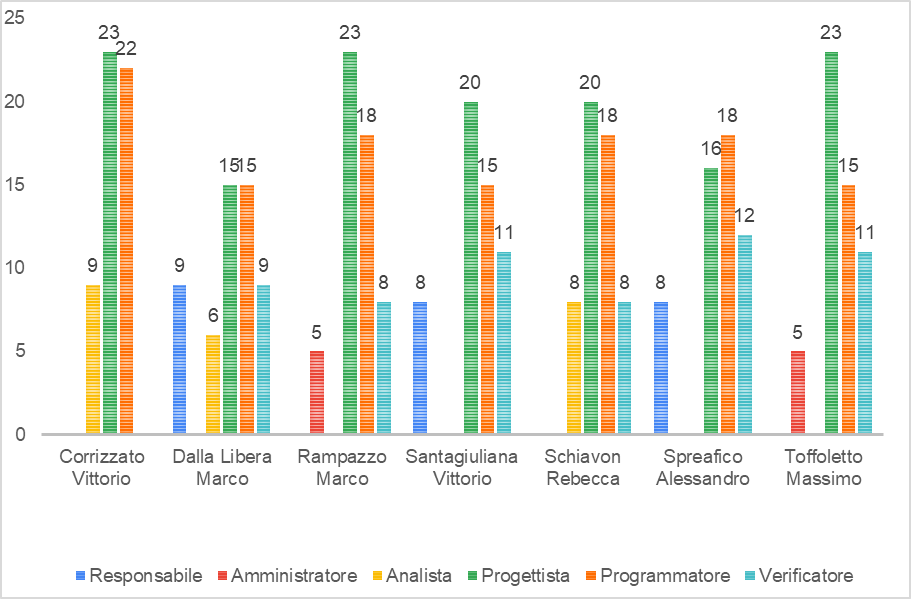
\includegraphics[width=\linewidth]{./img/Grafici/5.png}
\subsubsection{Prospetto economico}
Nel periodo di progettazione dettaglio e codifica sono previsti i seguenti costi:
\begin{longtable} {
		>{}p{32mm}
		>{}p{20mm}
		>{}p{20mm}
	}
	\rowcolor{gray!50}
	
	\textbf{Ruolo} & \textbf{Ore} & \textbf{Costo} \TBstrut \\
	Responsabile & 25 & 750 \TBstrut \\
	Amministratore & 10 & 200 \TBstrut \\
	Analista & 23 & 506 \TBstrut \\
	Progettista & 140 & 3080 \TBstrut \\
	Programmatore & 121 & 1815 \TBstrut \\
	Verificatore & 59 & 885 \TBstrut \\
	\textbf{Totale} & \textbf{378}& \textbf{7236} \TBstrut \\		
\end{longtable}
Rappresentati nel seguente grafico: \\
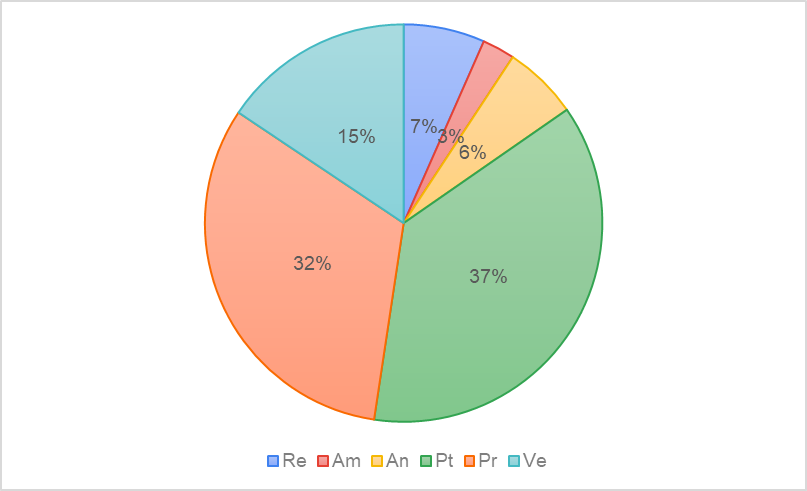
\includegraphics[width=\linewidth]{./img/Grafici/6.png}

\subsection{Periodo di validazione e collaudo}
\subsubsection{Prospetto orario}
Nel periodo di validazione e collaudo è prevista la seguente divisione oraria:
\begin{longtable} {				
		>{}p{40mm}  
		>{}p{8mm}
		>{}p{8mm}
		>{}p{8mm}
		>{}p{8mm}
		>{}p{8mm}
		>{}p{8mm}
		>{}p{12mm}			
	}			
	\rowcolor{gray!50}
	\textbf{Nominativo} & \textbf{Re} & \textbf{Am} & \textbf{An} & \textbf{Pt} & \textbf{Pr} & \textbf{Ve} & \textbf{Totale}	\TBstrut \\ [2mm]
	Corrizzato Vittorio & - & - & - & - & 10 & 10 & 20 \TBstrut \\ [2mm]
	Dalla Libera Marco & 8 & 5 & - & - & 7 & - & 20 \TBstrut \\ [2mm]
	Rampazzo Marco & - & - & - & 5 & 8 & 7 & 20 \TBstrut \\ [2mm]
	Santagiuliana Vittorio & - & 5 & - & - & 6 & 9 & 20 \TBstrut \\ [2mm]
	Schiavon Rebecca & - & 8 & - & - & 7 & 5 & 20 \TBstrut \\ [2mm]
	Spreafico Alessandro & - & - & - & - & 8 & 12 & 20 \TBstrut \\ [2mm]
	Toffoletto Massimo & - & - & - & - & 9 & 11 & 20 \TBstrut \\ [2mm]
\end{longtable}
Rappresentata nel seguente grafico: \\
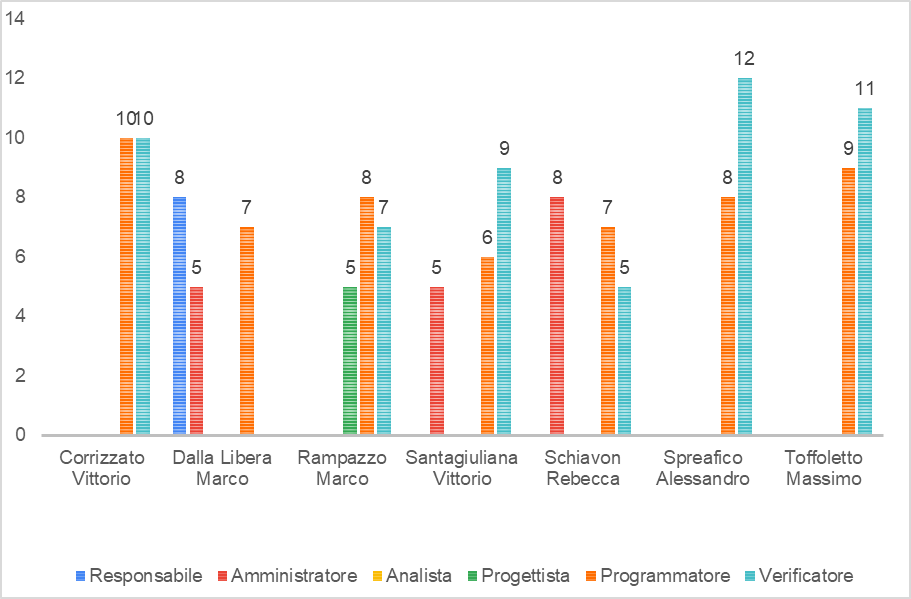
\includegraphics[width=\linewidth]{./img/Grafici/7.png}

\subsubsection{Prospetto economico}
Nel periodo di validazione e collaudo sono previsti i seguenti costi:
\begin{longtable} {
		>{}p{32mm}
		>{}p{20mm}
		>{}p{20mm}
	}
	\rowcolor{gray!50}
	
	\textbf{Ruolo} & \textbf{Ore} & \textbf{Costo} \TBstrut \\
	Responsabile & 8 & 240 \TBstrut \\
	Amministratore & 18 & 360 \TBstrut \\
	Analista & 0 & 0 \TBstrut \\
	Progettista & 5 & 110 \TBstrut \\
	Programmatore & 55 & 825 \TBstrut \\
	Verificatore & 54 & 810 \TBstrut \\
	\textbf{Totale} & \textbf{140}& \textbf{2345} \TBstrut \\		
\end{longtable}
Rappresentati nel seguente grafico: \\
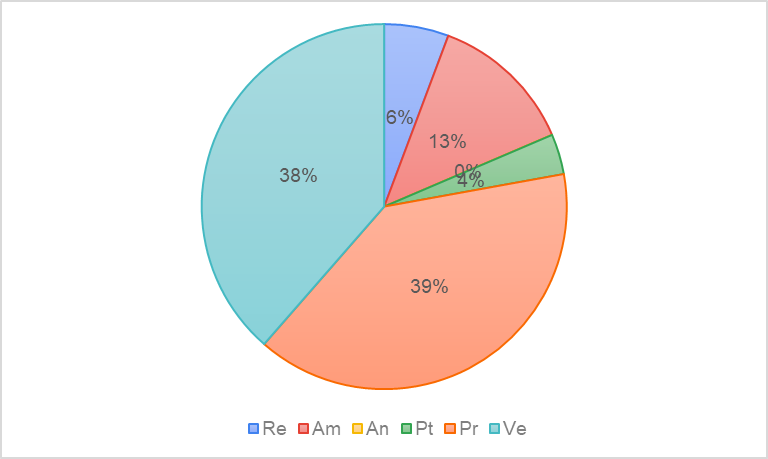
\includegraphics[width=\linewidth]{./img/Grafici/8.png}
	
\section{Consultivi di periodo}
Vengono riportati gli effettivi costi sostenuti per ogni periodo con le eventuali differenze rispetto a quanto preventivato. Il bilancio risulterà quindi:
\begin{itemize}
	\item \textbf{Positivo}: se i costi del consultivo risultano minori di quelli del preventivo;
	\item \textbf{Pari}: se i costi del consultivo risultano uguali a quelli del preventivo;
	\item \textbf{Negativo}: se i costi del consultivo risultano superiori a quelli del preventivo.
\end{itemize}
Seguiranno quindi le conclusioni con le motivazioni delle eventuali differenze e le contromisure che il gruppo ha deciso di attuare per evitare ulteriori discrepanze con quanto dichiarato nel preventivo.

	\subsection{Periodo di Analisi}
	La tabella riporta il numero di ore effettivamente svolte dal gruppo e il rispettivo costo con le eventuali differenze rilevate rispetto al preventivo.
	\begin{longtable} {							
			>{}p{40mm}  
			>{}p{20mm}	
			>{}p{28mm}			
		}			
		\rowcolor{gray!50}
		
		\textbf{Ruolo} & \textbf{Ore} & \textbf{Costo} \TBstrut \\
		Responsabile & 20 & 600 \TBstrut \\
		Amministratore & 25(-1) & 500(-20) \TBstrut \\
		Analista & 80(+9)& 1760(+198) \TBstrut \\
		Progettista & 21(+6) & 462(+132) \TBstrut \\
		Programmatore & 0 & 0 \TBstrut \\
		Verificatore & 43 & 645 \TBstrut \\
		\textbf{Totale Preventivo} & 175 & 3657	\TBstrut \\	
		\textbf{Totale Consultivo} & 189 & 3967	\TBstrut \\	
		\textbf{Differenza Totale} & 14 & 310 	\TBstrut \\	
	\end{longtable}

		\subsubsection{Conclusioni}
		Il bilancio risulta negativo perché le ore effettivamente svolte nei ruoli di analista, progettista e verificatore hanno superato le ore previste dal preventivo.
		Le motivazioni che hanno portato alla necessità di lavorare più del previsto sono le seguenti:
		\begin{itemize}
			\item Analisiti: la stesura dell'\textit{Analisi dei Requisiti} è risultata più complessa del previsto in particolare nell'individuazione dei casi d'uso e dei requisiti;
			\item Progettisti: sono sorte complicazioni non preventivate nella stesura del \textit{Piano di Qualifica} che hanno portato alla necessità di svolgere maggiore attività di autoapprendimento e ad un conseguente rallentamento del lavoro.
		\end{itemize}
		\subsubsection{Preventivo a finire}
		Il periodo di analisi è da intendersi come periodo di investimento per il gruppo e non viene quindi rendicontato, nel budget finale la variazione tra le ore previste e le ore effettive non provocherà alcun cambiamento. 
		È stato inoltre deciso di non modificare i successivi prospetti orari in quanto le condizioni che hanno portato alla necessità di lavorare più di quanto preventivato non dovrebbero presentarsi nuovamente. Il gruppo si ritiene ora più consapevole e meglio preparato, grazie anche alle ore di autoapprendimento già effettuate, e continua a considerare ragionevoli i prospetti orari dei prossimi periodi.
